\documentclass[a4paper, twocolumn, 11pt, oneside]{memoir}
\usepackage{preamble}

% Path for graphics
\graphicspath{{./graphics/}}

\title{Rutherford Scattering}
\author[1]{Kirsten A. Juhl \thanks{201606487@post.au.dk}}
\author[1]{Henriette Ravn  \thanks{20116112@post.au.dk}}
\author[1]{Laurits N. Stokholm \thanks{201605496@post.au.dk}}
\affil[1]{Department of Physics and Astronomy, Aarhus University}
\renewcommand{\Affilfont}{\itshape}
\date{\today}

% BibLateX
% style = authortitle
% nty
\usepackage[backend=biber, style=apa, defernumbers=true,
            sorting=nty, round]{biblatex}
\addbibresource{bibliography.bib}
\defbibheading{secbib}[\bibname]{%
    \section{#1}%
    \markboth{#1}{#1}}

%\raggedbottom
%\parindent = 0pt

%Følgende gør, at subscripts bliver ikke-kursiv. Anvendes X_|<subscript>|. Erstattes evt. med X_{\mathrm{<subscript>}}.
\makeatletter
\begingroup
\catcode`\_=\active
\protected\gdef_{\@ifnextchar|\subtextup\sb}
\endgroup
\def\subtextup|#1|{\sb{\textup{#1}}}
\AtBeginDocument{\catcode`\_=12 \mathcode`\_=32768 }
\makeatother

\DeclareSIUnit\gauss{G}

\begin{document}
% Dette er boksen i toppen. Lad den være.
%\vspace*{-13cm}
%\framebox[\textwidth][l]{\textbf{%
%\begin{tabular}{p{\linewidth}l}
%Received date: & {Approved:}\\
%& Date:\\
%& Signature:\\
%(reserved for instructor) & \\
%\end{tabular}
%}}
% Boksen slutter her .
%\vspace*{+1cm}
%\bigskip
% Title og Abstract
% Ignorerer twocolumn til abstract
\begin{minipage}{\textwidth}
    \twocolumn[
        \maketitle
        \begin{onecolabstract}
        \noindent
            This paper is written as the \emph{first} of four mandatory repports
during the course \emph{Experimental Physics III}.

In the experiment we will be working with ... 

At last ....

Hello from Kirstens computer (2nd time)

This resulted in ...
in confirmation of the theory

        \end{onecolabstract}]
\end{minipage}
\saythanks{}
%\vspace{9cm}
\section{Introduction} 
Almost all of our knowledge in the field of nuclear and atomic physics has been discovered through scattering experiments, and the theory of scattering underpins one of the most ubiquitous tools in physics.
In low energy physics, scattering phenomena provide the standard tool to
explore solid state systems. Historically, this was used as a first step
towards our current understanding of the atom.

This report examines the Rutherford scattering of a beam of
$\SI{350}{\kilo\electronvolt}$ protons on a thin foil of
a two layer $\mathrm{Au}$/$\mathrm{C}$ target. To limit the extend of the report, and to
keep our discussion simple and relevant, we will only examine elastic
collisions in the semi-classical regime, governed by the Sommerfeld criterion
for classical scattering \parencite[p. 14]{noteBB}.

This is usually fine for low energy physics, in which internal energies remain
constant and no further particles are created or annihilated.
For this experiment, which uses a single Van de Graaff accelerator to generate
particles with energies of up to $\SI{350}{\kilo\electronvolt}$, this is a good
approximation.

To safely guide the reader through this report with as little confusion as
possible a brief overview of the structure is given.
First, in section 2 the materials and methods are described. This leads to an
overview of the experimental setup and an in-depth review of both calibration
and startup procedure for the apparatus used in the experiment. Section 3 and 4
studies the angular dependency on cross section and proton energy, respectively.
Section 5 covers the determination of thickness of the target gold and carbon
layers. Finally, Section 6 gives a conclusion and reflection on the experiments.

%\section{Theory}
\subsection{Compton Scattering} Compton scattering occurs when a beam of
lightparticles, known as photons, collides with a solid target, in such a way
the photon collides with a bounded electron. The scattering process can be seen
on \cref{fig: comptonscattering}.  If the photon has an energy higher than the
binding energy of the electron, both the electron and the photon scatters. Then
the difference between the energy of the incomming and the scattered photon is
described by the Compton shift;
\begin{equation}
    \lambda - \lambda_0 = \frac{h}{m_ec}(1-\cos(\theta))
    \label{eq: comptonshift}
\end{equation}
Where $\lambda$ is the wavelength of the incoming photon, $\lambda_0$ is the
wavelength of the scattered photon, $h$ is Plancks constant, $m_e$ is the mass
of an electron, $c$ is the speed of light and $\theta$ is the angle in which
the photon is scattered. The derivation can be found in the \fxnote{appendix}.
Another effect closely related to this experiment is the photoelectric effect.
In contrast to the Compton effect, the photon energy is fully absorbed and goes
to two things; freeing the electron from its bounded state, and accelerating
the electron. The freed electron is called a photoelectron. This interaction
can of course not happen, if the photon do not have enough energy to free the
electron.

%\section{Hazards}
This experiment has primarily $3$ major hazards to be aware of, as listed below

\begin{itemize}
    \item High Voltage (HV). High severity, low risk. Turn off the power, and
        let it cool before switching it off on the O/I button. Especial care,
        if wearing a pacemaker or the alike.
    \item Lead poisoning. Low Severity, low risk. Do not touch the lead blocks.
        If necessary, use glows and wash hands. Do not eat or drink in the
        laboratory.
    \item Radioactivity. Low severity, low risk. Be careful when handling the
        radiation sources. Do not eat or drink in the laboratory. 
\end{itemize}

\section{Materials and Methods}
\subsection{Experimental Setup}
To obtain energies in the order of a $\SI{400}{\kilo\electronvolt}$, a single
Van-de-Graaf accelerator \cref{fig_setup3} was used. The variety of incomming
beam particles was limited by the source (a flask of hydrogen gas connected to
the accelerator tank), which was stationary and not changed. Therefore, we only
concider incomming ions $\mathrm{H^+}$ and $\mathrm{{H_2}^{+}}$. 
%
\begin{figure}[t]
    \centering
    \includegraphics[angle=-90, trim={35cm, 0cm, 27cm, 0cm}, clip,  width=0.99\columnwidth]{setup3}
    \caption{The Van-de-Graaf accelerator.}
    \label{fig_setup3}
\end{figure}
%
Acceleration of the ions was controllable by changing the voltage drop on the
dashboard \cref{fig_setup2} and thus also adjusting the kinetic energy of the
incoming beam. This will be described further in the section Procedure.

The beamline was placed in an angle relative to the accelerator. By changing
the magnetic field strength of the electromagnet, one could choose which of the
two possible incoming ions were deflected into the beamline and thus directed
towards scattering on the target material at the end of the beamline.

The motion of a charged particle in a magnetic field is governed by the Lorentz
force law, and as the trajectory of the motion is traced as part of a circle,
one obtains the necesarry equality for the motion to be\footnote{Concepts as
forces and spatial confinements to circular paths is meaningfull in the
classical regime. This is not the case for a fully relativistic and quantum
mechanical description.}

\begin{equation}
F_|m| = QvB = F_|cp| = \frac{mv^2}{r}.
\end{equation}
From this a ratio between the two magnetic fields needed for the respective
ions is
\begin{align}
    R_|B| = & \frac{B({\mathrm{H_2}^+})}{B(\mathrm{H^+})} =
    \frac{m({\mathrm{H_2}^+})
    v({\mathrm{H_2}^+})}{m(\mathrm{H^+})v(\mathrm{H^+})}\\
    & 2 \frac{v({\mathrm{H_2}^+})}{v(\mathrm{H^+})} = \sqrt{2}
\end{align}
%
where it has been assumed that the mass of the two ions are related by
$m(\mathrm{H^+}) = 2m(\mathrm{{H_2}^+})$ and the speed of each ion is given as
$v(\mathrm{X}) = \sqrt{\frac{2E}{m(\mathrm{X})}}$.
%
Given one of the magnetic fields, the other is determined from this ratio
factor. The following magnetic field strengths were used:
%
\begin{equation}
    B(\mathrm{H^+}) = \SI{1070}{\gauss} \quad B(\mathrm{{H_2}^+}) = \SI{1513}{\gauss}
\end{equation}
%
Conclusively, by changing the magnetic field strength, one changes the
incomming ion. BE AWARE: The magnetic field can change over the time scale of meassurements
due to mechanical heating of the metal in the electromagnet. This leads to expansion and thus
the magnetic field will be reduced.
%
\begin{figure}[t]
    \centering
    \includegraphics[width=0.99\columnwidth]{setup2}
    \caption{Overview of dashboard. Closer graphics are seen in the Procedure.}
    \label{fig_setup2}
\end{figure}
%
\begin{figure}[t]
    \centering
    \includegraphics[width=0.99\columnwidth]{setup1}
    \caption{Overview of detector and electromagnet (red brick).}
    \label{fig_setup1}
\end{figure}
%
\begin{figure}[t]
    \centering
    \includegraphics[trim={0cm, 10cm, 0cm, 40cm}, clip, width=0.99\columnwidth]{setup4}
    \caption{The equipment had a failure, so the targets were changed. We were
    lucky to get this picture of both detector and targets.}
    \label{fig_setup4}
\end{figure}
%
From the beamline the particles were directed toward a chosen target material
\cref{fig_setup4}, where they were scattered on atomic nuclei of the
target. A detector was placed at a movable position around the target, such
that scattering angles up $160$ degrees could be measured.

The detector was coupled to a digitizer connected to a computer. During
measurements the digitizer started a clock inside it. When the detector was hit
by a particle, the digitizer translated the measured energy into a digital
number and sent the number and the corresponding time stamp to the computer.
The program Mc2Analyzer was used to handle the data. The digital number is an
arbitrary number called a channel number. It is translatable to the actual
energy by a linear factor plus an offset. In order to convert these channel
numbers to correct energies of the scattered particles a calibration was done.

\subsection{Calibration}
An energy meassurement of the scattered ion gives a digitial output, which we call
a channel number (or bin number). These hold no physical interpretation, but
can be translated to the equivalent energy of the scattered particle. To
convert these channel numbers, a calibration is necesarry. 

Assuming a linear relationship between the energy and the channel number the
energy can be found as
\begin{equation}
    E = \alpha(k - k_|0|), \label{eq_calibration}
\end{equation}
where $k$ is the meassured channel, $k_0$ is the channelnumber corresponding to
a zero--amplitude input, and $\alpha$ is a conversion parameter.
The parameters in the relation is determined \cref{tab_parameters} by a two
step program.

\begin{table}[b]
\centering
\caption{The values of the parameters, used to convert channel numbers to
energies.}
\begin{tabular}{CC}
\toprule
\multicolumn{2}{c}{Calibration parameters}\\
\midrule
k_|0| & 1.36\pm 0.15 \\
\alpha & 0.800 \pm 0.005 \\
\bottomrule
\end{tabular}

\label{tab_parameters}
\end{table}

\subsubsection{Determing the zero-amplitude constant}
First, by connecting a pulser (variable output voltage), a relation between the
varied energy and the corresponding channel number is obtained. 
We did this for equidistant pulsed energies, and although unimportant for the
time being, we included the threshold input for a detected signal.

Data obtained can be plotted as count numbers versus bin numbers. Due to the
central limit theorem \parencite[p. 49]{statistics}, data can be fitted to a
gaussian distribution. This is done for each value of pulsed energy, for which
one gains parameter values for each gaussian within an uncertainty, determined
by the square root of covariance matrix diagonal \cref{fig_gaussian_fit}.

Each centroid (the mean bin number of the gaussian fit) was then compared as a
function of the pulser amplitude. As expected from \cref{eq_calibration}, this
shows a linear relation \cref{fig_linear_fit}.
The intersection is interpretated as the bin number for zero amplitude ($k_|0|$).
For values \cref{tab_parameters}.

\begin{figure}[t]
\centering
\includegraphics[width=0.99\columnwidth]{gaussian_fit}
\caption{Gaussian fits for all data meassured pulser-amplitude-signals. This was used to estimate the mean
bin number (centroid), and the uncertainty of the parameters used in the
energy-calibration.}
\label{fig_gaussian_fit}
\end{figure}

\begin{figure}[t]
\centering
\includegraphics[width=0.99\columnwidth]{k0_plotting}
\caption{Linear fit of the mean values as a function of amplitude. This was
used to determine the zero-amplitude constant $k_|0|$.}
\label{fig_linear_fit}
\end{figure}

 
\subsubsection{Determining alpha}
As described in the previous section, the magnetic field strength of the
electromagnet can be adjusted to deflect either $\mathrm{H^+}$ or
$\mathrm{{H_2}^+}$ into the beamline. For each of these a data point of energy
related to channel number can be found at a given angle.

The energy of the scattered particles, $E_|f|$, can be found by energy- and
momentum-conservation considerations for elastic scattering in two dimensions.
One is lead to the relation;
\begin{equation}
E_|f| = \left( \frac{m_|p| \cos\theta + \sqrt{{m_|t|}^2 - {m_|p|}^2
\sin^2\theta}}{m_|p|+m_|t|} \right)^2 E_|i|,
\label{eq_5}
\end{equation}
where $E_|i|$ is the energy of the incident beam particles, $m_|p|$ and $m_|t|$ are
the masses of the incident protons and the target particles, respectively, and
$\theta$ is the angle between the direct outgoing non-scattered beam and the
scattered particles - also called the scattering angle.

Unfortunately, this only give two data points one from $\mathrm{H^+}$ and
another from $\mathrm{{H_2}^+}$. Nonetheless, the incline from the linear fit
to these data points is still useful. We however found a work around solution
for this specific problem. By using a target of two layers; gold and carbon
respectively, we have multiple centroids; one for $\mathrm{H_2^+}$ and the gold
layer, another two for $\mathrm{H^+}$
scattering off both gold and carbon \cref{fig_gaussian_fit2}. Thus the linear fit
\cref{fig_linear_fit2} has a third point.

One should be aware of the difference between the two linear fits. First we
fitted for two parameters, both incline and intersection, and obtained the
value of the zero-amplitude bin value \cref{fig_linear_fit}. Afterwards, we fitted for a single
parameter, the incline, and used the value of $k_|0|$ \cref{fig_linear_fit2}.

\begin{figure}[t]
\centering
\includegraphics[width=0.99\columnwidth]{gaussian_fit2}
\caption{From left to right we see $\mathrm{H_|2|^{+}}$ scattering off the gold layer
and $\mathrm{H^+}$ scattering off the carbon and gold layer respectively.}
\label{fig_gaussian_fit2}
\end{figure}

\begin{figure}[t]
\centering
\includegraphics[width=0.99\columnwidth]{alpha_plotting}
\caption{A linear fit of three points.}
\label{fig_linear_fit2}
\end{figure}

\subsection{Targets}
\fxnote{FIX}
The targets of interest in this experiment was a thin gold coated carbon plate. The gold coating was about one tenth of the carbon thickness. The thickness of the carbon plate have previously been determined as $\SI{250}{\angstrom}$, and the thickness of the gold coating as $\SI{25}{\angstrom}$.\footnotemark \footnotetext{The estimated thickness of each target available have been determined by the previous users of the experimental setup and written down on the whiteboard next to the setup.} 
The target was placed in holder, which contains several other targets. The height of the holder was fixed, though it was not investigated whether the marked height was optimal with respect to the beam position.\\

When measuring proton scattering at different angles, the blind angles of the
target holder may cause a problem. In order to avoid the targets "blind-spots",
the target was turned at an angle following the detector while still avoiding
the incoming proton beam to hit a blind angle. The blind angles of the holder
are around $\pm \SI{30}{\degree}$ in each side of the target holder, see figure .  



%\subsection{Scattering on atomic nuclei}
%The aim of this experiment was to use a particle accelerator to test certain dependencies of Rutherford scattering. Numerically, the Rutherford scattering differential cross section per target atom for any target atom is
%\begin{equation}
%\frac{d\sigma}{d\Omega} = 1.296 \left( \frac{Z_1 Z_2}{E_\infty [MeV] \, \sin^2 \left(\frac{\theta}{2} \right) }\right)^2\left[\frac{mb}{sr}\right],
%\end{equation}
%where $\theta$ is the scattering angle, $Z_1$  is the atomic number of the incident particles, $Z_2$ is the atomic number of the target nuclei, and $E_{\infty}$ is their kinetic energy HUSK CITE!%cite 
%. 
%In order to test these dependencies a relation between the cross section and the count rate (number of scattered particles per time) is found as
%\begin{equation}
%dN = N \, n_{\text{tar}} \, dx \,d\Omega \, \frac{d\sigma(\theta,\phi)}{d\Omega},
%\end{equation}
%where $N$ is the number of incoming particles per time, $n_\text{tar}$ is the particle density of the target, $dx$ is the thickness of the target, and $d\Omega$ is the solid angle of the detector.
%

\clearpage
\subsection{Procedure}
For a complete description of the experimental setup, we have provided this
short review of the startup procedure. This can be omitted, but found valueable
for the course examination.

First thing, the Van-de-Graaf. To accelerate the beam of incomming particles,
one has to generate a hugh potential. Turning on the Belt, one hears the
mechanical rhumming. This will generate a potential difference as described
further in \cite[p. 565]{krane}.
\begin{figure}[h!]
\centering
\includegraphics[trim={0, 45cm, 0, 15cm}, clip, width=0.9\columnwidth]{process1}
\caption{The belt is turned on.}
\label{fig_process1}
\end{figure}

Now adjust the terminal voltage patiently towards the wanted energy. Our lab
instructor advised us to wait for each step, before going to the next.
\begin{figure}[h!]
\centering
\includegraphics[trim={0, 20cm, 0, 55cm}, clip, width=0.9\columnwidth]{process2}
\caption{Terminal voltage is adjusted to $\SI{350}{\kilo\electronvolt}$.}
\label{fig_process2}
\end{figure}

Turn on the electromagnet. One can dial in the calculated magnetic field
strength wanted. This will do absolutely nothing, but translate the origin of
the scale. To do actual change of the magnetic field strength, one has to
change the current throught the electromagnet.
\begin{figure}[h!]
\centering
\includegraphics[trim={0, 30cm, 0, 30cm}, clip, width=0.9\columnwidth]{process3}
\caption{Dashboard for the electromagnet.}
\label{fig_process3}
\end{figure}

Now open the vacuum valve, so the incomming ions can be detected.
If the Faraday cup (detector for $0$ degree scatter) is connected to an Ampere
meter, one can look for received current of charged particles. This should be
maximized, by a variational principle about the calculated magnetic field,
using the fine grid for adjustments.

\begin{figure}[h!]
\centering
\includegraphics[trim={0, 35cm, 0, 30cm}, clip, width=0.9\columnwidth]{process4}
\caption{Ampere meter connected to the Faraday cup to detect current of charged
particles detected.}
\label{fig_process4}
\end{figure}
When the signal is good, there is one last step which is to set the output of
the faraday cup from the Ampere meter to the input of the collector. This will
give a precise count for the detected ions picked up in the faraday cup.
\begin{figure}[b]
\centering
\includegraphics[trim={35cm, 0cm, 0cm, 25cm}, clip, width=0.9\columnwidth]{process5}
\caption{Collector with a timer. This can be set to stop counting after a time
interval.}
\label{fig_process5}
\end{figure}








\section{Thickness of the target layers} 
Most of the particles pass directly through the target without scattering. However, a small amount do scatter. When particles pass through the first layer they loose energy. As a consequence, there will be a difference in the energy of the particles entering the first and the second layer. 

By comparing measurements of scattering on the target with gold layer facing the beam and the carbon layer facing the beam, the distributions for scattering on carbon and gold are observed at different energies. 

\begin{figure}[h]
\centering
\includegraphics[width=0.99\columnwidth]{tykkelse.png}
\caption{Sketch of how to determine thickness of the target carbon layer from the energy difference between: a) gold layer facing the beam and b) carbon layer facing the beam.}
\label{fig_sketch_thickness}
\end{figure}


%The energies of the scattered protons is due to the ratio between the mass of the protons and the mass of the target. 
The energy differences are proportional to the thickness of target layers. To determine the thickness of the carbon layer we consider what happens to the energy in the two following situations. In situation a) gold is facing the beam, and the final energy is given as the incoming energy minus the energy lost due to scattering on gold:
\begin{equation*}
Ea_f = E_i (1-f_E(\theta)), 
\end{equation*}
where $f_{Au}(\theta)$ is the function giving the relation between the incoming energy $E_i$ and the particle energy $E_f$ in equation \cref{eq:5} after scattering on gold. 
In situation b) carbon is facing the beam, and the final energy is given as the incoming energy minus the energy lost due to the following: passing through the carbon layer, scattering on gold, and passing through the carbon layer again on the way out. 
\begin{align*}
Eb_f &= E_i - t_\mathrm{C} \left(\frac{dE}{dx}\right)_\mathrm{C} 
\\ &- f_E(\theta) \left(E_i - t_\mathrm{C} \left(\frac{dE}{dx}\right)_\mathrm{C} \right) \\ &- \frac{t_\mathrm{C}}{\cos(\pi-\theta)} \left(\frac{dE}{dx}\right)_\mathrm{C}, 
\end{align*}
where $\left(\frac{dE}{dx}\right)_\mathrm{C}$ is the stopping power of carbon found in the table in the laboratory.

The energy change for the peak position of the distribution for gold is found as the difference between the two situations. Thus, the thickness of the carbon layer is found as 
\begin{equation}
t_\mathrm{C} = \frac{\Delta E_{\mathrm{Au}}}{\left(\frac{dE}{dx}\right)_\mathrm{C} \left(1 - f_\mathrm{Au}(\theta) - \frac{1}{\cos(\theta)} \right)}
\end{equation}



%The thickness of the gold layer is found using the same approach for gold.
%\begin{equation}
%\Delta E_{Au} = t_C \left(\frac{dE}{dx}\right)_C \left(1 - f_E(\theta) + %\frac{1}{\cos(\pi-\theta)} \right),
%\end{equation}



\begin{figure}[t]
\centering
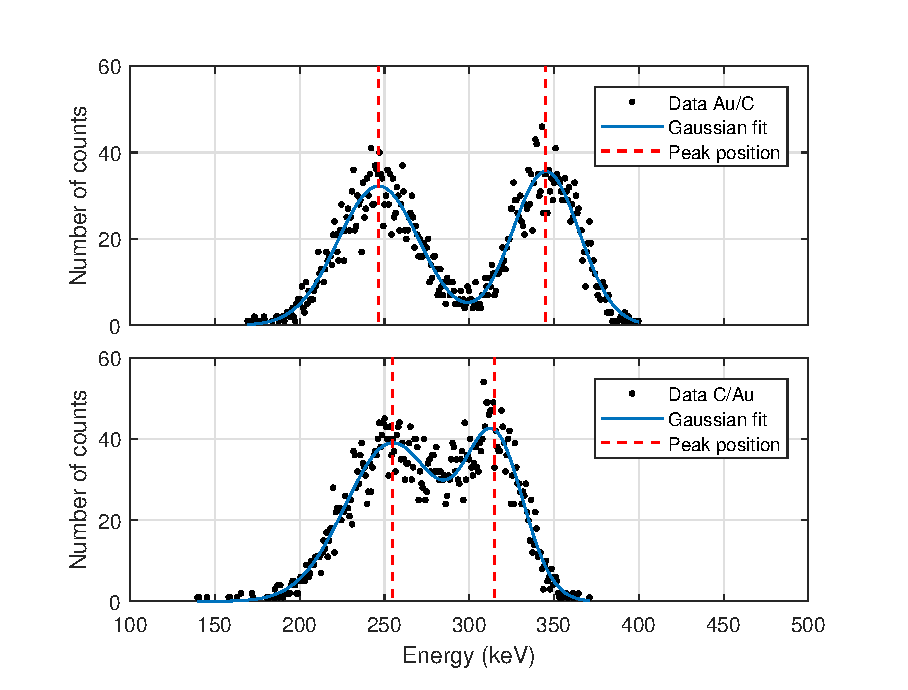
\includegraphics[width=0.99\columnwidth]{Dterminethicknessplot.eps}
\caption{Thickness of target layers determined from change in energy. Upper: gold layer facing the beam. Lower: carbon layer facing the beam.}
\label{fig_thickness}
\end{figure}




%\section{Discussion}
%
%\subsection{The experimental setup}
%The Van de Graaf accelerator provide an enormous advantage over the
%Cockcroft-Walton accelerator as the terminal voltage on a Van de Graaf is
%extreemely stable and does not ripple as the later does. This is very important
%when desired to measure reaction cross sections. Nonetheless, the Van de Graaf
%accelerator has a low current output in the $\si{\micro\ampere}$ range compared
%with the Cockcroft-Walton $\si{\milli\ampere}$. Nevertheless, this is quite
%sufficient for nuclear reaction experiments, and thus our chosen accelerator is
%the workhorse of low-energy nuclear structure physics.
%
%To improve the potential drop across the accelerator:
%
%Vacuum, so the limit of electrical breakdown (sparking) of 
%
%To reduce breakdown and sparking, the generator is enclosed in a pressure tank
%containing an insulating gas.
%Capacitance (geometrical size)
%\cite{krane}
%
%\subsection{Rutherford experiment}
%
%Provide data that test the angular dependence of the Rutherford cross section for scattering of 400kV protons on gold and carbon
%Measure the energy of the scattered protons on gold and carbon as a function of scattering angle 
%Provide data that test the Ztarget dependence of the Rutherford cross section
%Measure the thickness of the gold and carbon layers in the target.
%Challenge tasks :
%Provide data that checks the energy dependence of the Rutherford cross section
%Demonstrate that nuclear reactions occur when protons are incident on boron
%The measurement plan should as a minimum include 
%
%Calibration of the detector by using a pulser and one measured energy from the accelerator, or by using H+ and H2+ beams (do not direct the beam directly into the detector!).
%A plan to achieve the required tasks 1-4.
%
%Target dependency of the Rutherford cross section
%Nuclear reactions of protons with boron.


\section{Conclusion}
During the experiment the Rutherford scattering has been examined. A relation between the differential cross section have been determined and compared with the theory assuming that the Summerfeld criterion is fulfilled. 


The classical Rutherford scattering of low energy hydrogenic ions, $H^+$ and $H_2^+$ on a double layered target of $\SI{20}{\angstrom}$ gold and $\SI{200}{\angstrom}$ carbon have been examined. Especially the angular dependency of the scattered particles was investigated. 


There is a clear relation between the fit of the data counts and the deviation of the theoretical expected energies.  

Accordingly, two gaussians; one for carbon and another for gold, was fitted. For small angles the two gaussians merged, making the estimation of the centroid more difficult. For larger angles, this problem is avoided. Another problem occur. We see a small bump in between the carbon and gold gaussians. Thus our assumption of a double gaussian is bad. This could be dodged had we fitted a tripple gaussian, which might shift the the carbon centroid towards higher bins and thus a higher energy. 



We assumed a linear combination of the two gaussian distributions. Nonetheless, this might have lead to 


\clearpage
\printbibliography[heading=subbibliography]{}
\nocite{*}
\end{document}

